\section{Redes SOM}\label{som}
Mapas auto-organizáveis (Self-Organized Maps) ou Mapas de Kohonen são um tipo de rede neural. Foram desenvolvidos em 1982 por Tuevo Kohonen, professor emérito da Academia da Finlândia. ``Auto-organização'' é porque a supervisão não é
necessária. SOMs aprendem por conta própria através da aprendizagem competitiva não supervisionada. ``Mapas'' significa que eles tentam mapear seus pesos para entrar em conformidade com os determinados dados de entrada. Os nós de uma rede SOM tentam tornar-se igual às entradas que lhes são apresentados. Neste sentido, é assim que eles aprendem.

\subsection{Estrutura}

A Figura \ref{fig:som-node} é uma rede SOM 4x4 (4 linhas por 4 colunas de neurônios). Cada mapa está ligado a cada nó de entrada. Para esta pequena rede 4x4, resulta em 4x4x3 = 48 ligações. 

Nota-se que os nós da camada de saída do mapa não são ligados uns aos outros. Os nós organizados desta maneira, como uma grade de duas dimensões, faz com que seja fácil de visualizar os resultados. 

Nesta configuração, cada nó tem um única coordenada (i, j), tornando mais fácil fazer referência a um nó na rede, e calcular as distâncias entre os nós. Devido as ligações serem apenas dos nós de saída para o nós de entrada, os nós da camada de saída são indiferentes quanto ao valores dos pesos de seus vizinhos. A atualização dos pesos será explicada em sequência \ref{treinamento}.

\begin{figure}[ht]
\centering
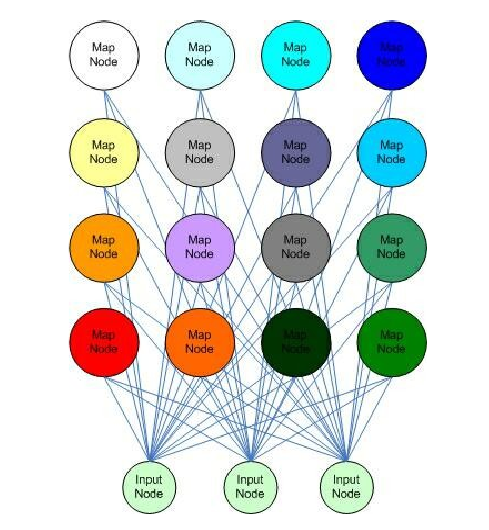
\includegraphics[scale=0.5]{imgs/node-som.png}
\caption{Nó do Mapa de Kohonen}
\label{fig:som-node}
\end{figure}